\chapter{Runtime View (Dynamic View)}

\section{System Initialization}
\label{sec:system_initialization}
\Requirement{017}
{The API shall perform TCS initialization.}
{\Satisfies{SRS_TCS 020}}

\Requirement{018}
{TCS will have an initialization routine invoked by BswM or initialization runnable and this is decided by the configuration parameter \code{TcsGenerateInitRunnable}. 
When the configuration parameter is set to TRUE, the initialization is done by the  \RunnableRef{Runnable_TCS_Init} that calls the static  \code{TCS_Init}, otherwise the initialization is done by the global  \code{TCS_Init}, called by the BswM Init rule.}
{\Satisfies{SRS_TCS 021} \Satisfies{SRS_TCS 020}}

\Requirement{027}
{\Function{TCS_Init}
{\code{void}}{}{}
{\code{void}}
{This function is responsible for:
\begin{itemize}
\item Initializing the output port to initial value
\item Transitioning the execution state of the SUM_TCS module
\end{itemize}
}
}
{\Satisfies{SRS_TCS 029}}

\section{System De-initialization}
N/A

\section{Detailed Design}

\subsection{Macros}
\label{sec:macros}

\Requirement{028}
{\Macro{TCS_RESETREQUEST_MASK}
{0x40}
{Bitmask used to identify the ECU Reset Requested flag bit in the \code{SUSD_TCS_PermitExecution} interface.
The ECU Reset Requested flag is bit 6.}}
{\Satisfies{SRS_TCS 013}}

\Requirement{029}
{\Macro{TCS_ENABLE_SHUTDOWN}
{255u}
{Value corresponding to \code{Enable} for the \code{TCS_SUSD_ShutdownPermission} interface.}}
{\Satisfies{SRS_TCS 013}}

\Requirement{030}
{\Macro{TCS_SHUTDOWN_CNT_LIMIT}
{4u}
{Upper limit for the alive counter transmitted with the \code{TCS_SUSD_ShutdownPermission} interface command \code{SUSD_UserRequest}.
This behaviour is described in the SUM_SUSD requirements in SDV-8002.}}
{\Satisfies{SRS_TCS 012}}

\subsection{Data Types}
\label{sec:data_types}

\Datatype{TimeSyncMessageType}
{\code{uint64}}
{A 64-bit unsigned integer containing a TimeSyncMessage}

%\subsection{Structures}
%N/A

%\subsection{Enums}
%N/A

%\section{Wakeup procedure}
%N/A

%\section{Sleep procedure}
%N/A

%\section{Boot loading procedure}
%N/A

%\section{Failure handling strategy}
%N/A

\section{Critical timing constraints}
\begin{itemize}
\item The periodicity of \RunnableRef{Runnable_TCS_MasterClockPolling} must be less than or equal to the transmission rate of the \code{TimeSyncMessage} received by the Time Leader.
\item The periodicity of \RunnableRef{Runnable_TCS_TimeManagement} must be a submultiple of the resolution of the \code{TimeSyncMessage} (100 ms).
\end{itemize}

\section{Task management}

\subsection{Periodic Runnables}
\label{sec:periodic_runnables}

\Requirement{001}
{\RunnableRef{Runnable_TCS_MasterClockPolling} shall use a variable \code{EA_LocalTimeClock} to keep a local time source and synchronize with Master Clock signal.}
{\Satisfies{SRS_TCS 001}}

\Requirement{003}
{\RunnableRef{Runnable_TCS_MasterClockPolling} shall receive the MasterClockSignal.}
{\Satisfies{SRS_TCS 003} \Satisfies{SRS_TCS 027}}

\Requirement{006}
{\code{SumTCSInitValue} should be first initialized to zero.}
{\Satisfies{SRS_TCS 006}}

\Requirement{013}
{\RunnableRef{Runnable_TCS_MasterClockPolling} shall check the validity of the received MasterClockSignal based on the value of MasterClockSignalAvailability.}
{\Satisfies{SRS_TCS 015}}

\Requirement{019}
{\RunnableRef{Runnable_TCS_MasterClockPolling} shall implement the local time counter with same resolution as of the timestamp and synchronize the same with the reception of every valid Time Sync signal.}
{\Satisfies{SRS_TCS 022} \Satisfies{SRS_TCS 028}}

\Requirement{020}
{\RunnableRef{Runnable_TCS_MasterClockPolling} should record the last clock local value into the variable \code{SumTCSInitValue}.}
{\Satisfies{SRS_TCS 023}}

\Requirement{026}
{\RunnableRef{Runnable_TCS_MasterClockPolling} shall consume the time sync signal.}
{\Satisfies{SRS_TCS 030}}

\Requirement{034}
{\RunnableRef{Runnable_TCS_MasterClockPolling} shall support multiple TimeSyncMessage reception modes: service-based (ComSignal) and signal-based (ComSignal or ComGroupSignal), determined by configuration parameters.}
{}

\Runnable{Runnable_TCS_MasterClockPolling}
{Fixed}
{EA_LocalTimeClock

EA_SubCounter
}
{MasterClockSignal

MasterClockSignalAvailability}
{}
{}
{\code{void}}
{This runnable is responsible for:
\begin{itemize}
\item Polling new Master Clock signal and availability signal
\item Synchronizing local timer to Master Clock
\end{itemize}
The TimeSyncMessage reception mode is determined by the configuration:
\begin{itemize}
\item \textbf{Service-based} (SOME/IP): when \code{TCS\_ServiceBased\_TimeSyncMessage\_Ref} is configured and \code{comSignalType} is \code{UINT8\_N}, the signal is read via a ComSignal as a service data element with transformer error handling. The received byte array is converted to \code{uint64} via \code{TCS\_Prv\_byteArray\_to\_uint64}.
\item \textbf{Signal-based ComGroupSignal}: when \code{TCS\_TimeSyncMessageSignalRef} references a ComGroupSignal with \code{comSignalType} \code{UINT64}, the signal is read via a signal group struct. When E2E is configured, the \code{Rte\_Read} call includes a \code{Rte\_TransformerError} parameter.
\item \textbf{Signal-based ComSignal} (default): when \code{TCS\_TimeSyncMessageSignalRef} references a ComSignal with \code{comSignalType} \code{UINT64}, the signal is read directly as a \code{uint64} value.
\end{itemize}
}
{\Satisfies{SRS_TCS 001} \Satisfies{SRS_TCS 003}}

\Requirement{011}
{\RunnableRef{Runnable_TCS_TimeManagement} shall increment the variable \code{EA_SubCounter} during each period of execution as long as the \code{PermitExecution} notification is active.}
{\Satisfies{SRS_TCS 011}}

\Requirement{015}
{\RunnableRef{Runnable_TCS_TimeManagement} shall update \code{EA_LocalTimeClock} to ensure it meets \code{SumTCSGlobalTimePrecision}.}
{\Satisfies{SRS_TCS 016}}

\Requirement{016}
{\code{EA_LocalTimeClock} payload shall match the payload of the MasterClock signal.}
{\Satisfies{SRS_TCS 022}}

\Runnable{Runnable_TCS_TimeManagement}
{Fixed}
{EA_LocalTimeClock

EA_SubCounter
}
{}
{TCS_SWC_Clock}
{}
{\code{void}}
{This runnable is responsible for:
\begin{itemize}
\item Keeping  a local clock source to maintain the time between Master Clock Signal receptions
\item Providing a local clock source
\end{itemize}
}

\Requirement{009}
{\RunnableRef{Runnable_TCS_PermitExecutionShutdown} shall monitor \code{PermitExecution} input in order to execute.}
{\Satisfies{SRS_TCS 009}}

\Requirement{024}
{\RunnableRef{Runnable_TCS_PermitExecutionShutdown} shall set \code{TCS_SUSD_ShutdownPermission} to \code{Enable} when the ECU Reset bit in the \code{SUSD_TCS_PermitExecution} value is \code{FALSE} after checking that there are no pending NVM writes.}
{\Satisfies{SRS_TCS 013}}

\Requirement{010}
{\RunnableRef{Runnable_TCS_PermitExecutionShutdown} shall allow execution of all functions when the Wakeup(s) Active bit in the \code{PermitExecution} interface is \code{TRUE} and not set to \code {FALSE} even when wakeup(s) is no longer
active.\newline
The below image shows the state machine of \RunnableRef{Runnable_TCS_PermitExecutionShutdown}.


\begin{center}
	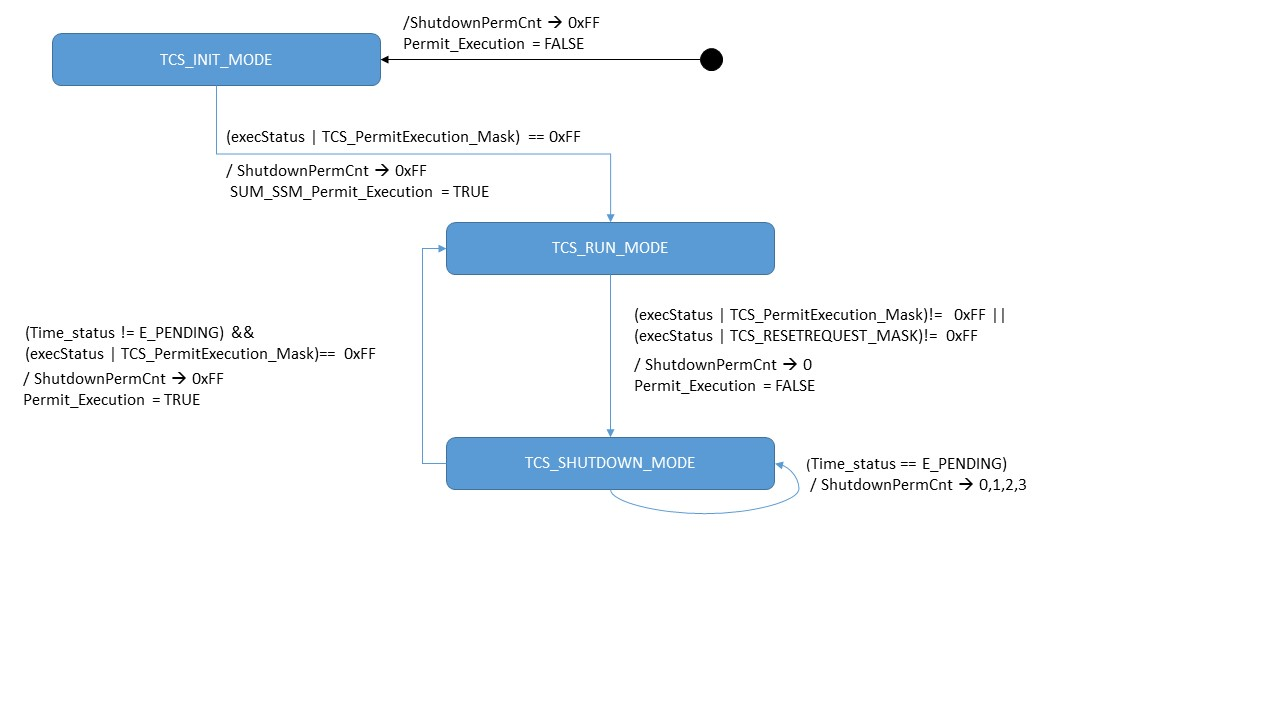
\includegraphics[scale=0.45]{images/State_Machine}
\end{center}


}
{\Satisfies{SRS_TCS 010}}

\Requirement{032}
{\RunnableRef{Runnable_TCS_PermitExecutionShutdown} shall write the RAM mirror block \code{SumTCSInitValue} into NVM during the power-down process. Write operation shall be prevented if the battery voltage is not good to perform it, by checking \code{BatteryVoltage_DisableNVMWrite} from SUSD.}
{\Satisfies{SRS_TCS 023}}

\Requirement{005}
{\code{SumTCSInitValue} should be retrieved before starting the SUM_TCS module and use to substitute the last received value following initialization.}
{\Satisfies{SRS_TCS 005}}

\Requirement{007}
{\code{EA_LocalTimeClock} shall be initialized with the value of the RAM mirror block \code{SumTCSInitValue} which is retrieved from NvM during initialization of the SUM_TCS module.}
{\Satisfies{SRS_TCS 007}}

\Runnable{Runnable_TCS_PermitExecutionShutdown}
{Fixed}
{EA_LocalTimeClock

EA_SubCounter}
{SUSD_TCS_PermitExecution

RP_SUSD_TCS_BatteryVoltage_DisableNVMWrite}
{TCS_SUSD_ShutdownPermission

TCS_SWC_Clock}
{}
{\code{void}}
{This runnable is responsible for:
\begin{itemize}
\item Handling execution and shutdown permissions
\item Only once when first allowing execution:
\begin{itemize}
\item Initializing \code{EA_LocalTimeClock} and \code{TCS_SWC_Clock} by reading \code{SumTCSInitValue} from NVM
\item Initializing \code{EA_SubCounter} to zero
\end{itemize}
\end{itemize}
}

\Requirement{033}
{When the configuration parameter \code{TcsGenerateInitRunnable} is set to TRUE, the initialization is done by the  \RunnableRef{Runnable_TCS_Init} that calls the static \code{TCS_Init}.}
{\Satisfies{SRS_TCS 020}}

\Runnable{Runnable_TCS_Init}
{Fixed}
{EA_LocalTimeClock}
{}
{TCS_SWC_Clock}
{}
{\code{void}}
{This runnable is responsible for for calling the \code{TCS_Init} function.}
\clearpage

\subsection{Triggered Runnables}
\label{sec:trig_run}
\Requirement{008}
{\RunnableRef{Runnable_TCS_Dem_Clock} is called each time a local clock is needed for DEM time stamping.}
{\Satisfies{SRS_TCS 008}}

\Runnable{Runnable_TCS_Dem_Clock}
{Event}
{EA_LocalTimeClock}
{}
{TCS_Dem_Clock}
{}
{\code{Std_ReturnType}}
{This runnable is responsible for:
\begin{itemize}
\item Providing the timestamp to Dem when needed for a DTC event
\end{itemize}
}

\Requirement{021}
{\RunnableRef{TCS_TotalVehicleTimeRead} is called each time the Total Vehicle Time value is needed.}
{\Satisfies{SRS_TCS 014} \Satisfies{SRS_TCS 024} \Satisfies{SRS_TCS 025}}

\Runnable{TCS_TotalVehicleTimeRead}
{Event}
{}
{}
{}
{}
{\code{Std_ReturnType}}
{This runnable is responsible for:
\begin{itemize}
\item Providing the Total Vehicle Time value
\end{itemize}
}

\Runnable{TCS_TotalVehicleTimeCheckRead}
{Event}
{EA_LocalTimeClock}
{}
{}
{}
{\code{Std_ReturnType}}
{Function for condition check read of Total Vehicle Time value.}

\section{Runtime Scenario}

\subsection{Initialization}

SUM_TCS has two states, \code{INIT} and \code{RUN}.
The \code{INIT} state is entered during startup and when the initialization function has been called.
The \code{RUN} state is entered only when the \code{PermitExecution} interface flags are set to enable.
There is no shutdown state, rather each runnable shall monitor the \code{PermitExecution} flag to determine when to begin shutting down the module.

\begin{figure}[h]
	\centering
	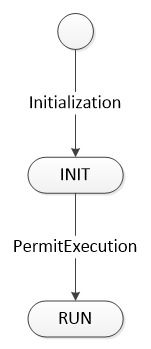
\includegraphics[scale=0.7]{images/state.png}
	\caption{SUM_TCS state diagram}
\end{figure}

\clearpage
\subsection{Runnables and communication}
\label{sec:communication}

\UMLDiagramModified{generated/diagrams/TCS_Communication}{Overview of TCS communication}{0.45}
